\documentclass[12pt,a4paper]{article}

\usepackage[T1]{fontenc}
\usepackage[brazilian]{babel}
\usepackage{lmodern}
\usepackage{microtype}
\usepackage[a4paper,margin=2.5cm]{geometry}
\usepackage{graphicx}
\usepackage{booktabs}
\usepackage{tabularx}
\usepackage{array}
\usepackage{float}
\usepackage{longtable}
\usepackage{hyperref}
\usepackage{xurl}
\usepackage{enumitem}
\usepackage{caption}

\hypersetup{
  colorlinks=true,
  linkcolor=blue,
  urlcolor=blue,
  citecolor=blue,
  pdftitle={Estudo Experimental de Desempenho de HTTP/1.1, HTTP/2 e HTTP/3},
  pdfauthor={Kleber Moura de Jesus}
}

\setlength{\parindent}{1.25cm}
\setlength{\parskip}{0.25em}
\renewcommand{\arraystretch}{1.15}
\graphicspath{{results/20261020T205948Z-881/plots/}}

\title{
  \textbf{Estudo Experimental de Desempenho de Protocolos Web}\\
  \large HTTP/1.1, HTTP/2 e HTTP/3 em Ambiente Emulado
}
\author{
  Kleber Moura de Jesus\\
  Universidade Federal do Piauí -- CSHNB\\
  Redes II
}
\date{20 de outubro de 2026}

\begin{document}
\maketitle

\begin{center}
\textbf{Vídeo de apresentação (15 minutos):} link não listado do YouTube a inserir após a gravação.
\end{center}

\begin{abstract}
Este trabalho compara HTTP/1.1 sobre TCP, HTTP/2 protegido por TLS 1.3 sobre TCP e HTTP/3
sobre QUIC em dois cenários de rede emulados. São avaliadas a transferência de um objeto de
50 MB e a transferência concorrente de 100 objetos de 10 KB. O cliente registra o tempo até
o primeiro byte do corpo (TTFB), tempos de resposta, duração total da carga, requisições por
segundo (RPS), percentis e bytes recebidos. Foram executadas duas rodadas completas de
T01--T12, com cinco repetições por teste. Os resultados mostram que o desempenho depende
da carga e do cenário: HTTP/3 teve vantagem na transferência grande sob WAN na segunda
rodada, mas não foi o mais rápido em todos os testes. A análise considera a multiplexação,
o bloqueio de início de linha, a variabilidade entre repetições e as limitações das
implementações utilizadas.
\end{abstract}

\noindent\textbf{Palavras-chave:} HTTP/1.1; HTTP/2; HTTP/3; QUIC; TCP; desempenho; \texttt{tc netem}.

\section{Introdução}

HTTP/1.1, HTTP/2 e HTTP/3 oferecem semânticas de aplicação semelhantes, mas diferem no
transporte, no estabelecimento seguro de conexão e na multiplexação. Essas decisões podem
alterar a latência de início, a vazão e a cauda da distribuição de latência, sobretudo quando
há RTT alto e perda de pacotes. O objetivo deste estudo é medir essas diferenças de maneira
reprodutível, mantendo fixos os perfis de conteúdo e a emulação do caminho.

O experimento não presume que um protocolo será sempre superior. A interpretação distingue
custo de handshake, transferência de um objeto grande, concorrência de objetos pequenos,
implementação concreta dos servidores e variação entre repetições.

\section{Fundamentação teórica}

\subsection{HTTP/1.1 e HTTP/2 sobre TCP}

HTTP/1.1 utiliza TCP e, neste ensaio, não utiliza TLS. Uma conexão TCP nova exige o
estabelecimento do transporte antes da troca de dados da aplicação. O ensaio de carga A
abre uma conexão nova por amostra para que a latência inicial inclua esse custo. Para a
carga B, o cliente mantém uma conexão persistente; HTTP/1.1 não multiplexa respostas
independentes no mesmo canal como HTTP/2, e o limite de uma conexão no pool deixa visível
a serialização das respostas.

HTTP/2 mantém a semântica de HTTP sobre TLS 1.3/TCP e multiplexa streams por quadros na
mesma conexão. Isso elimina o bloqueio de aplicação próprio da sequência de respostas do
HTTP/1.1, mas não elimina a entrega ordenada do TCP. Uma perda de segmento pode atrasar
a entrega dos bytes subsequentes da conexão, inclusive bytes pertencentes a outros streams.

\subsection{TCP CUBIC -- Tanenbaum \S 6.5.11}

TCP CUBIC ajusta a janela de congestionamento usando uma função cúbica do tempo desde o
último evento de congestionamento. Após detectar perda, o algoritmo reduz a janela e tenta
retomar o crescimento de forma mais rápida perto do valor de janela anterior, mantendo uma
curva de crescimento mais suave quando se afasta daquele ponto. Em uma WAN emulada com
perdas estocásticas, perdas repetidas podem provocar novas reduções antes de a janela
recuperar o nível necessário para preencher o caminho. O RTT também aumenta o tempo
necessário para receber confirmações e retransmitir dados. A consequência esperada é a
redução da vazão TCP útil em T04 e T05, não porque a cifragem TLS altere o algoritmo CUBIC,
mas porque ambos dependem de TCP e enfrentam a mesma perda do caminho. A magnitude dessa
diferença é resultado experimental.

Essa interpretação depende da implementação e do sistema operacional do servidor que envia
os dados. O comportamento de controle de congestionamento não pode ser atribuído apenas ao
cliente HTTP nem inferido da porcentagem nominal de perda; deve ser tratado como uma
explicação compatível com o mecanismo TCP observado.

\subsection{QUIC e BBR -- Tanenbaum \S\S 6.6.1--6.6.2}

QUIC integra TLS 1.3 ao estabelecimento de transporte sobre UDP e oferece streams
independentes. Diferentemente da entrega ordenada global do TCP, a perda de dados de um
stream QUIC não exige que dados já recebidos de outros streams aguardem a retransmissão
daquele stream. Essa propriedade reduz o bloqueio de início de linha (HoL blocking) entre
streams de HTTP/3, mas não elimina bloqueios dentro do mesmo stream, perdas, retransmissões
ou contenção de congestionamento compartilhado pela conexão.

O BBR estima a largura de banda do gargalo e o RTT mínimo para controlar o ritmo de envio,
em vez de usar cada perda isolada como único sinal de congestionamento. Esse princípio pode
ajudar a explicar resiliência em enlaces com perdas não necessariamente causadas por
congestionamento. Contudo, QUIC não implica que BBR esteja ativo: o algoritmo selecionado
depende da implementação do servidor QUIC. Como a configuração e a versão usadas neste
experimento não confirmaram BBR, não se atribuem a esse algoritmo os resultados de T06,
T09 ou T12.

\section{Metodologia}

\subsection{Ambiente e controle experimental}

O ambiente é composto por Nginx servindo HTTP/1.1 e HTTP/2 com TLS 1.3, Caddy servindo
HTTP/3/QUIC e um cliente Python assíncrono. Os quatro contêineres pertencem à rede bridge
\texttt{172.20.0.0/16}. O cliente também está na bridge para que o atraso configurado em sua
saída e na saída dos servidores forme o caminho de ida e volta. Na LAN aplica-se 0,5 ms em
cada sentido e nenhuma perda. Na WAN aplicam-se 25 ms de atraso em cada sentido e 2\% de
perda somente na saída dos servidores, evitando somar duas taxas de perda de 2\%.

O runner gera um certificado autoassinado de laboratório com SAN para os nomes dos serviços,
gera objetos com bytes pseudoaleatórios para reduzir efeitos de compressibilidade, constrói
e inicia os contêineres, executa a matriz, salva os dados, gera os gráficos e remove os
contêineres e as disciplinas \texttt{tc}. O certificado é confiável pelo cliente via arquivo
de CA; a validação do certificado não é desativada.

Na carga A, cada amostra cria e fecha uma sessão de cliente/conexão antes da próxima medição.
Assim, o TTFB inclui o estabelecimento de TCP/TLS ou QUIC. Na carga B, cada repetição mantém
uma única conexão de transporte por protocolo, e os 100 pedidos são submetidos
concorrentemente por essa conexão. HTTP/1.1 é limitado a uma conexão e serializa as respostas;
HTTP/2 e HTTP/3 podem multiplexar streams. O cliente solicita \texttt{no-cache} e
\texttt{no-store}, não implementa cache, e os servidores enviam \texttt{Cache-Control:
no-store}.

Cada teste tem cinco repetições. Os gráficos exibem média e desvio-padrão entre repetições.
Média, mediana e desvio-padrão de TTFB são calculados sobre as cinco médias por amostra;
p50 e p99 de TTFB e duração individual são calculados sobre os registros de requisições.
Para Carga B, há 500 requisições individuais por teste (100 em cada uma de cinco repetições).
Para Carga A, há somente cinco observações individuais por teste, portanto seus percentis
empíricos são pouco precisos. RPS e tempo total da carga são estatísticas das cinco amostras
agregadas.

\subsection{Matriz experimental}

\begin{table}[H]
\centering
\small
\caption{Matriz dos doze testes realizados.}
\begin{tabularx}{\textwidth}{@{}l l l l X@{}}
\toprule
Teste & Carga & Protocolo & Rede & Foco analítico\\
\midrule
T01 & 1 $\times$ 50 MB & HTTP/1.1 & LAN & Vazão TCP sem perda\\
T02 & 1 $\times$ 50 MB & HTTP/2 + TLS 1.3 & LAN & TLS e TCP cifrado\\
T03 & 1 $\times$ 50 MB & HTTP/3 & LAN & QUIC sem perda\\
T04 & 1 $\times$ 50 MB & HTTP/1.1 & WAN & RTT e perda em TCP\\
T05 & 1 $\times$ 50 MB & HTTP/2 + TLS 1.3 & WAN & TCP/TLS sob perda\\
T06 & 1 $\times$ 50 MB & HTTP/3 & WAN & QUIC sob perda\\
T07 & 100 $\times$ 10 KB & HTTP/1.1 & LAN & Serialização de respostas\\
T08 & 100 $\times$ 10 KB & HTTP/2 + TLS 1.3 & LAN & Multiplexação HTTP/2\\
T09 & 100 $\times$ 10 KB & HTTP/3 & LAN & Streams QUIC\\
T10 & 100 $\times$ 10 KB & HTTP/1.1 & WAN & RTT/perda e serialização\\
T11 & 100 $\times$ 10 KB & HTTP/2 + TLS 1.3 & WAN & Perda TCP e multiplexação\\
T12 & 100 $\times$ 10 KB & HTTP/3 & WAN & Streams QUIC sob perda\\
\bottomrule
\end{tabularx}
\end{table}

\subsection{Métricas}

O TTFB registrado é o intervalo, em microssegundos, desde o início do pedido até o primeiro
byte do corpo da resposta. Ele inclui estabelecimento de conexão nos testes frios. O tempo
de resposta individual mede até o último byte do objeto; o tempo total da carga mede a janela
completa da amostra. RPS é o total de respostas bem-sucedidas dividido por essa janela.
Os percentis p50 e p99 de latência são calculados sobre tempos individuais de resposta.

\subsection{Registro das execuções}

Foram realizadas duas execuções completas em 20 de outubro de 2026. Cada rodada contém
cinco repetições para cada um dos doze testes (60 amostras agregadas por rodada), além dos
registros brutos por requisição.

\begin{table}[H]
\centering
\small
\caption{Execuções preservadas e respectivos artefatos.}
\begin{tabularx}{\textwidth}{@{}l l l X@{}}
\toprule
Rodada & Identificador & Cobertura & Artefatos\\
\midrule
1 & \texttt{20261020T194130Z-578} & T01--T12, 5 repetições/teste &
\href{results/20261020T194130Z-578/results.json}{JSON};
\href{results/20261020T194130Z-578/results.csv}{CSV};
\href{results/20261020T194130Z-578/plots/summary.md}{resumo}\\
2 & \texttt{20261020T205948Z-881} & T01--T12, 5 repetições/teste &
\href{results/20261020T205948Z-881/results.json}{JSON};
\href{results/20261020T205948Z-881/results.csv}{CSV};
\href{results/20261020T205948Z-881/plots/summary.md}{resumo}\\
\bottomrule
\end{tabularx}
\end{table}

Os diretórios e arquivos de cada rodada foram preservados separadamente. As rodadas são
reportadas individualmente, sem combinar amostras nem selecionar apenas a rodada mais
favorável. As diferenças entre rodadas são apresentadas como variação observada entre
execuções, não como estimativa estatística independente de dez repetições.

\section{Resultados}

Os gráficos da segunda rodada apresentam média e desvio-padrão entre as cinco repetições.
A Tabela~\ref{tab:comparison} compara métricas agregadas selecionadas; os valores após
$\pm$ são desvios-padrão entre repetições, não intervalos de confiança.

\begin{table}[H]
\centering
\caption{Comparação selecionada entre as duas rodadas.}
\label{tab:comparison}
\begin{tabular}{@{}lrr@{}}
\toprule
Teste e métrica & Rodada 1 & Rodada 2\\
\midrule
T03 -- tempo total da carga A (s) & $4{,}207 \pm 1{,}026$ & $3{,}824 \pm 0{,}214$\\
T06 -- tempo total da carga A WAN (s) & $114{,}292 \pm 7{,}292$ & $110{,}153 \pm 4{,}624$\\
T08 -- RPS da carga B LAN & $161{,}87 \pm 28{,}87$ & $248{,}05 \pm 24{,}13$\\
T09 -- RPS da carga B LAN & $192{,}66 \pm 29{,}20$ & $225{,}10 \pm 6{,}41$\\
T12 -- RPS da carga B WAN & $53{,}99 \pm 34{,}11$ & $94{,}05 \pm 37{,}86$\\
\bottomrule
\end{tabular}
\end{table}

Na segunda rodada, HTTP/3 apresentou menor tempo médio de carga que HTTP/1.1 e HTTP/2 em
T06. Em LAN, T09 teve RPS médio inferior ao HTTP/2 em T08, embora superior ao T09 da
primeira rodada. Em WAN, T12 teve RPS médio maior na segunda rodada, mas sua dispersão
entre repetições continua alta. Os resultados variam com o cenário e a carga e não sustentam
a afirmação de que HTTP/3 seja sempre mais rápido.

\begin{figure}[H]
\centering
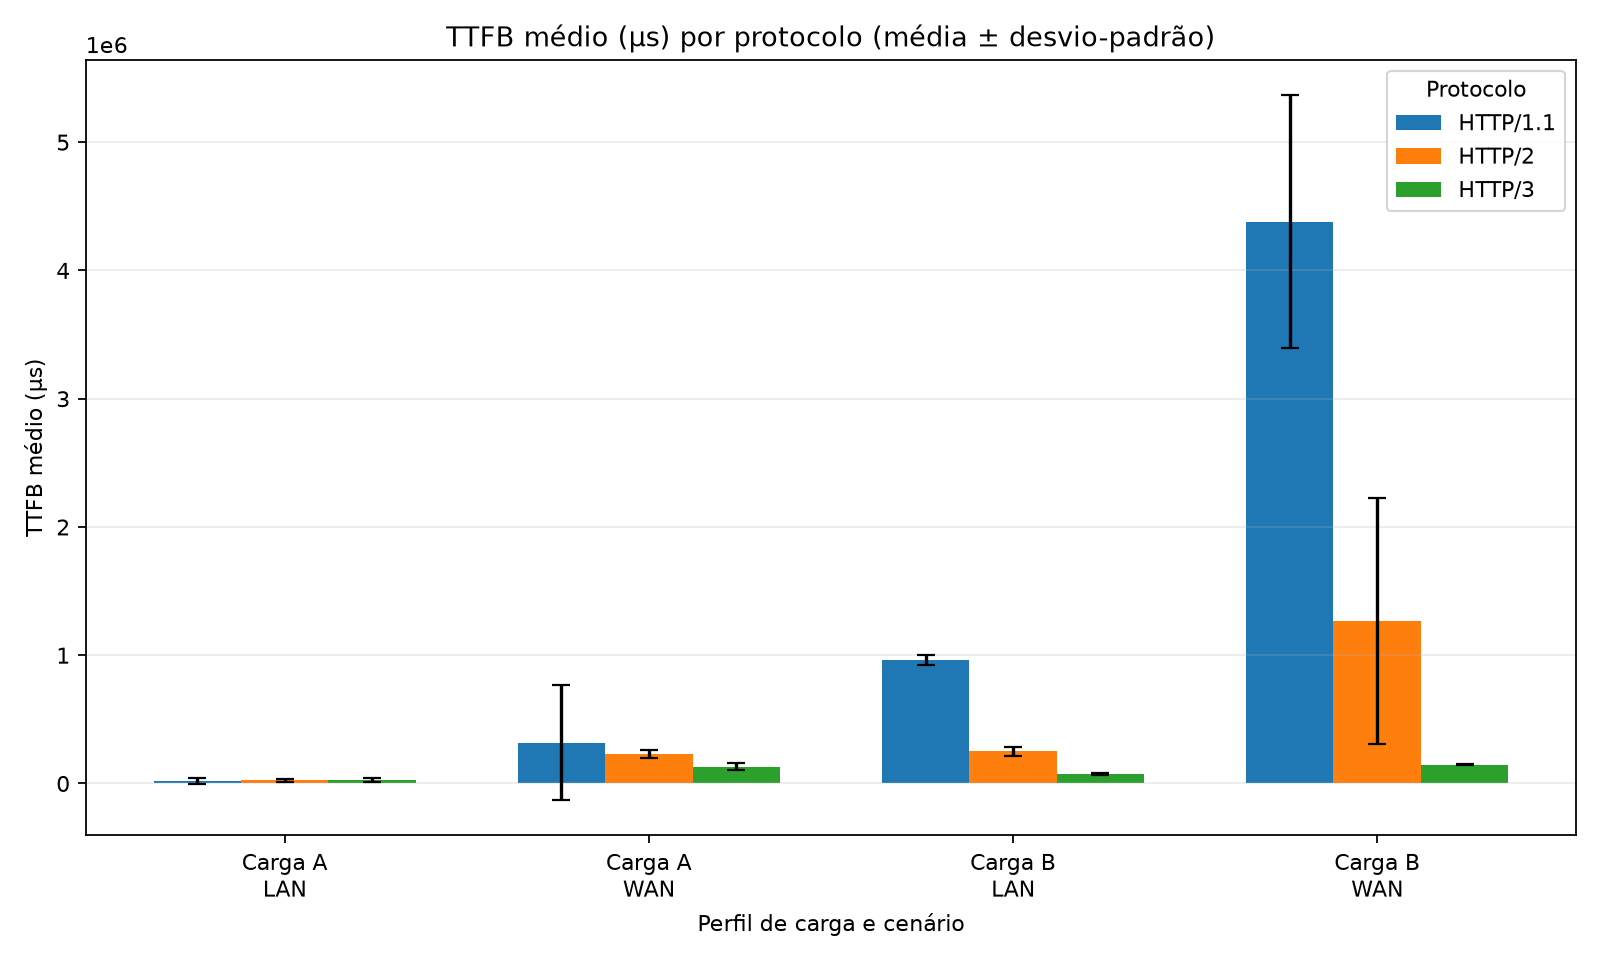
\includegraphics[width=0.88\textwidth]{ttfb.png}
\caption{TTFB por protocolo, carga e cenário na segunda rodada. Barras de erro: $\pm$ um
desvio-padrão entre cinco repetições.}
\label{fig:ttfb}
\end{figure}

\begin{figure}[H]
\centering
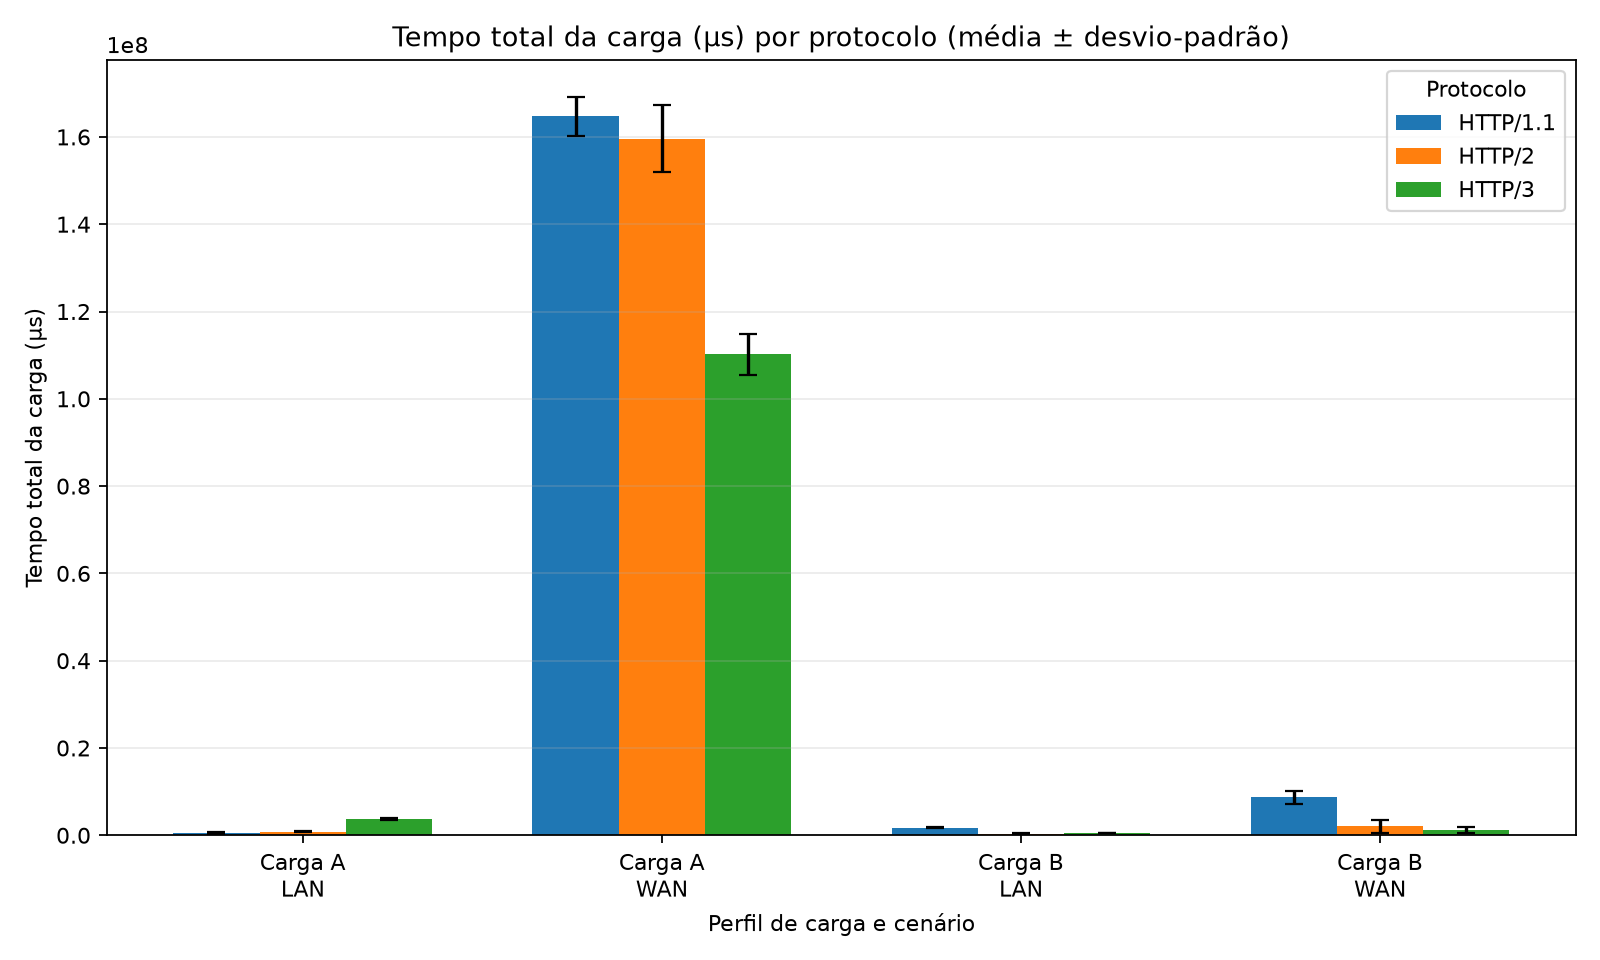
\includegraphics[width=0.88\textwidth]{total_load.png}
\caption{Tempo total da carga por protocolo, carga e cenário na segunda rodada. Barras de
erro: $\pm$ um desvio-padrão entre cinco repetições.}
\label{fig:total}
\end{figure}

\begin{figure}[H]
\centering
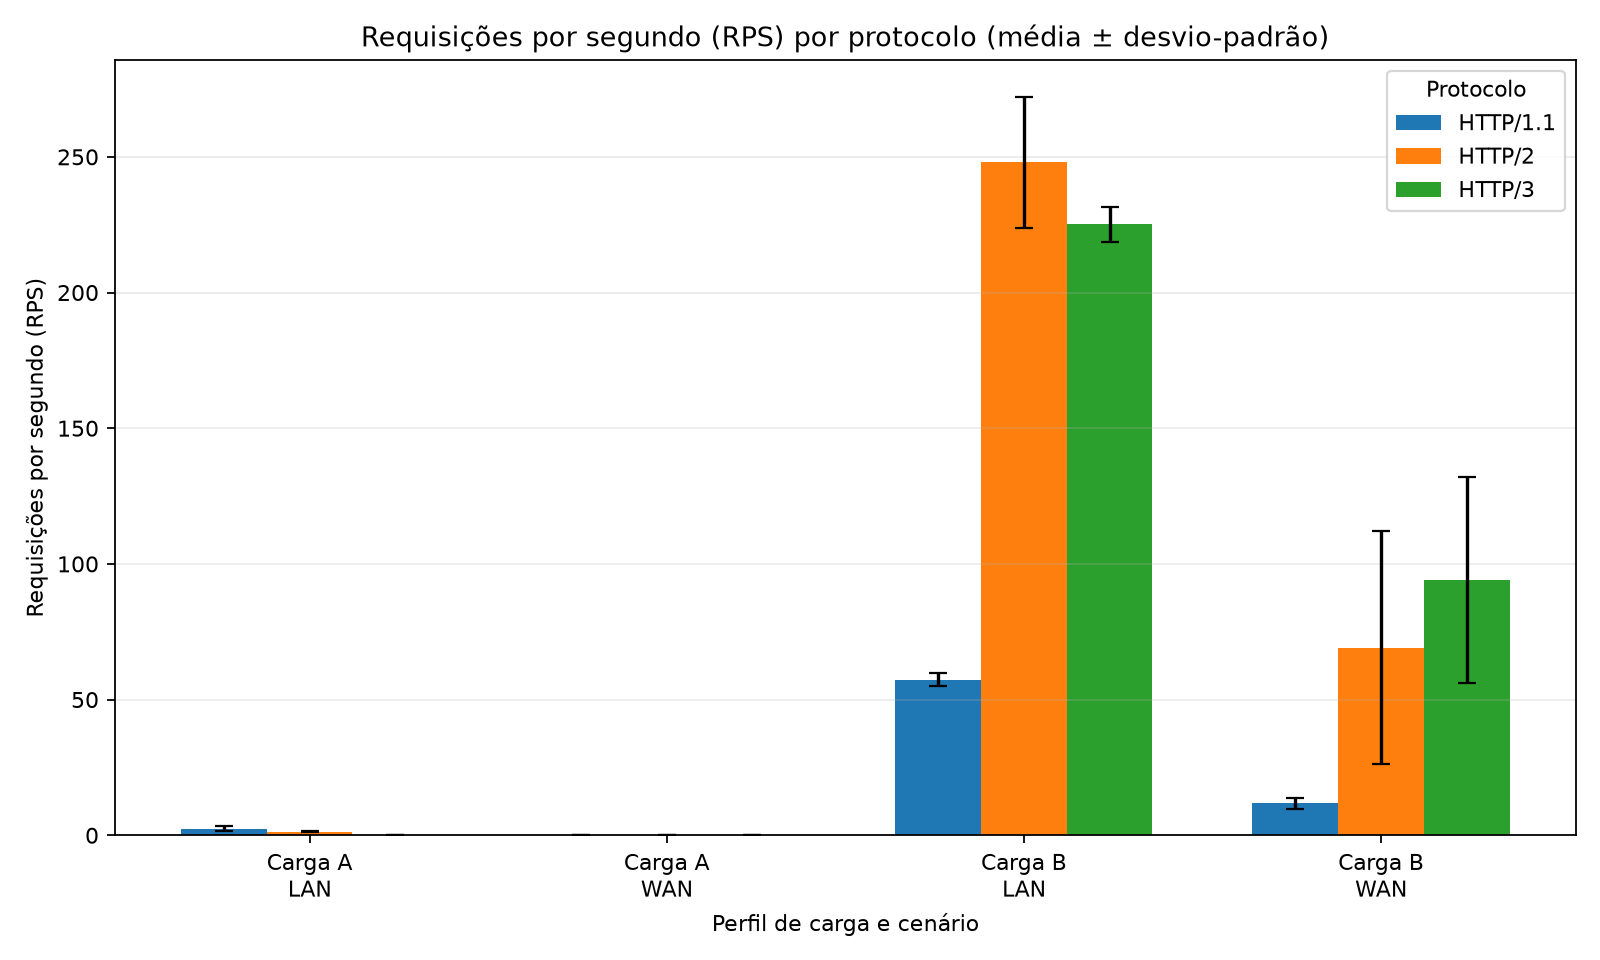
\includegraphics[width=0.88\textwidth]{rps.png}
\caption{RPS por protocolo, carga e cenário na segunda rodada. Barras de erro: $\pm$ um
desvio-padrão entre cinco repetições.}
\label{fig:rps}
\end{figure}

As tabelas estatísticas completas, incluindo percentis de latência calculados a partir dos
registros individuais, estão nos arquivos
\href{results/20261020T194130Z-578/plots/summary.md}{summary da rodada 1} e
\href{results/20261020T205948Z-881/plots/summary.md}{summary da rodada 2}.

\section{Discussão}

\subsection{Handshake e TTFB}

Os testes de Carga A criam uma conexão nova por requisição, de modo que o TTFB observado
inclui o estabelecimento da conexão e o tempo até o primeiro byte do corpo. Na segunda
rodada, as médias de TTFB em LAN foram aproximadamente 19,9 ms (T01), 24,8 ms (T02) e
26,2 ms (T03). Em WAN foram 318,9 ms (T04), 228,1 ms (T05) e 131,4 ms (T06). A menor
média de TTFB de WAN em T06 é compatível com menor latência inicial para QUIC nesse ensaio,
mas não isola o custo do handshake: também inclui processamento no servidor, escalonamento,
transporte dos dados e variação entre as cinco observações. Em LAN, HTTP/3 não apresentou
o menor TTFB médio nesta rodada. Portanto, os dados não demonstram uma vantagem uniforme
de TTFB em todos os cenários.

Os p50/p99 para Carga A têm somente cinco observações individuais por teste, uma por
repetição. Esses percentis são descritores empíricos muito instáveis e não devem ser
interpretados como estimativas precisas da cauda de latência. Para Carga B, os percentis
agregam 500 pedidos, mas os pedidos pertencem a cinco lotes concorrentes e não são 500
observações independentes.

\subsection{Objeto grande e transporte}

Para um objeto de 50.000.000 bytes, o tempo médio da segunda rodada em LAN foi 0,477 s em
T01, 0,771 s em T02 e 3,824 s em T03. Isso corresponde aproximadamente a 105, 65 e 13 MB/s,
respectivamente, usando MB decimal e o tempo médio da carga. O resultado de T03 mostra que
esta implementação HTTP/3/aioquic foi bem mais lenta que as implementações TCP no cenário
LAN de objeto grande. Ele não prova que QUIC como protocolo seja intrinsecamente mais lento:
diferenças de implementação, cópias e processamento em espaço de usuário, configuração e
limites do host podem contribuir.

Na WAN, os tempos médios foram 164,739 s (T04), 159,564 s (T05) e 110,153 s (T06), ou
aproximadamente 0,304, 0,313 e 0,454 MB/s. HTTP/3 teve maior vazão efetiva e menor duração
neste conjunto. A configuração injetou 2\% de perda na saída dos servidores e 25 ms de atraso
em cada sentido. A forte diferença entre LAN e WAN é compatível com o impacto de RTT e perda
na recuperação de transporte. É coerente discutir CUBIC para T04/T05 se o kernel Linux de fato
usou o algoritmo padrão esperado, mas o experimento não registrou diretamente o algoritmo
TCP ativo nem a evolução da janela de congestionamento. Assim, a associação com CUBIC é uma
interpretação teórica, não uma variável medida.

Em Carga A há somente uma requisição por amostra; o campo RPS é essencialmente o inverso
da duração daquela transferência e não é uma métrica apropriada para comparar vazão de
objeto grande. Para essa carga, tempo total e bytes transferidos são mais informativos.

\subsection{Objetos pequenos, multiplexação e HoL}

Na segunda rodada em LAN, a carga concorrente alcançou cerca de 57 RPS em T07, 248 RPS em
T08 e 225 RPS em T09. HTTP/2 superou HTTP/3 em RPS médio neste cenário, enquanto HTTP/3
teve o menor TTFB de requisição (p50 aproximado de 71,6 ms contra 279,5 ms em HTTP/2).
Isso indica que as métricas não apontam um vencedor único: HTTP/3 iniciou as respostas mais
rapidamente no conjunto medido, mas o lote HTTP/2 completou mais requisições por segundo.
HTTP/1.1 ficou atrás, resultado compatível com a serialização sobre uma conexão limitada a
um canal.

Na WAN, T10/T11/T12 registraram aproximadamente 11,8, 69,2 e 94,0 RPS, respectivamente.
O TTFB p50 por requisição foi aproximadamente 4,15 s, 0,762 s e 0,149 s. O padrão é
compatível com custo de RTT e serialização em HTTP/1.1, com multiplexação em HTTP/2, e com
streams independentes de QUIC reduzindo o bloqueio entre streams. Ainda assim, T12 teve
desvio-padrão de cerca de 37,9 RPS entre repetições e p99 de duração individual de cerca de
2,12 s, indicando dispersão e eventos de cauda relevantes. A independência de streams não
elimina perda, retransmissão ou controle de congestionamento compartilhado pela conexão.

\subsection{Variação entre rodadas e limites de inferência}

As duas rodadas concordam qualitativamente que HTTP/1.1 tem desempenho inferior na carga
concorrente WAN (T10) e que HTTP/3 foi mais rápido que os dois protocolos TCP para o objeto
grande WAN (T06). Outros resultados variaram: T08 subiu de 162 para 248 RPS entre rodadas,
enquanto T09 passou de 193 para 225 RPS; em T12, HTTP/3 passou de 54 para 94 RPS, com
dispersão elevada em ambas as rodadas. Essa variação pode refletir escalonamento, estado do
host, operações em segundo plano e aleatoriedade de perdas. Como as rodadas não foram
planejadas como um ensaio controlado de repetibilidade, elas são reportadas separadamente e
não foram agregadas como se fossem dez repetições equivalentes.

O BBR não foi configurado nem verificado na imagem Caddy usada; portanto, não é possível
atribuir os resultados HTTP/3 a BBR. A explicação suportada pelos dados é limitada à
implementação de HTTP/3/QUIC executada e à propriedade arquitetural de isolamento entre
streams.

\section{Limitações e reprodutibilidade}

O experimento compara implementações concretas (Nginx, Caddy e aioquic/httpx), não
implementações abstratas dos padrões. O cliente aioquic e os servidores Caddy/Nginx não são
a mesma pilha de implementação, e o algoritmo de congestionamento usado por QUIC não foi
verificado. O \texttt{tc netem} é aplicado à saída das interfaces dos contêineres, de modo que
tráfego de controle e de aplicação também pode ser afetado. Os 2\% são uma probabilidade de
perda por pacote na saída dos servidores, não uma taxa constante de perda de bytes. O caminho
de contêineres não representa toda a variabilidade da Internet real.

As execuções ocorreram no Docker Desktop para Windows com backend Linux/WSL2, em uma
máquina reportada pelo Docker com quatro CPUs e aproximadamente 3,8 GiB disponíveis. A
versão do cliente Docker/Compose informada durante a execução foi 29.5.2/5.1.4. As imagens
Nginx e Python usam tags móveis (\texttt{alpine} e \texttt{3.12-slim}) e as dependências
Python têm faixas de versão, sem lockfile; isso limita a reprodução binária exata. O
identificador de imagem Caddy no Compose é \texttt{2.7-alpine}. Para reprodução futura
rigorosa, devem ser registrados os digests das imagens e as versões efetivamente resolvidas
dos pacotes.

Para reproduzir, em Linux com Docker Compose, OpenSSL e permissões para executar Docker
(ou Docker Desktop com Git Bash no Windows):
\begin{verbatim}
chmod +x run_experiments.sh scripts/*.sh
REPETITIONS=5 ./run_experiments.sh
\end{verbatim}

O runner salva os dados brutos em JSON e CSV e os gráficos e a tabela consolidada no
diretório de resultados identificado pelo horário UTC da execução. A automação encerra os
contêineres e remove \texttt{tc qdisc} também em caso de falha. Os artefatos gerados devem
ser preservados junto com as anotações do ambiente experimental.

\section{Conclusão}

Nas condições testadas, os resultados não mostram um protocolo vencedor para todas as cargas.
HTTP/3 apresentou o menor tempo médio para transferir o objeto grande na WAN (T06, cerca de
110 s, contra 160--165 s em TCP) e o maior RPS médio na carga concorrente WAN da segunda
rodada (T12, cerca de 94 RPS). Em contrapartida, HTTP/3 teve o maior tempo para o objeto
grande em LAN (T03, cerca de 3,82 s), e HTTP/2 alcançou maior RPS que HTTP/3 na carga
concorrente LAN da segunda rodada (T08 versus T09). HTTP/1.1 teve o menor RPS nos testes
de objetos pequenos, especialmente na WAN.

Esses resultados são compatíveis com benefícios de multiplexação e isolamento de streams em
algumas condições, mas também evidenciam o custo de implementação e a variabilidade. Cinco
repetições por teste, sobretudo cinco observações para latência da carga A, não bastam para
caracterizar com precisão caudas raras ou provar significância estatística. A explicação
baseada em TCP CUBIC é teoricamente pertinente, mas o algoritmo e a janela ativa não foram
medidos; da mesma forma, não se comprovou o uso de BBR em QUIC. Portanto, as conclusões
se restringem às versões e ao ambiente documentados e não devem ser extrapoladas para todos
os servidores, clientes ou redes reais.

\begin{thebibliography}{9}
\bibitem{tanenbaum}
TANENBAUM, Andrew S.; WETHERALL, David J.
\textit{Redes de Computadores}. 5. ed. São Paulo: Pearson Prentice Hall, 2011.
Seções 6.5.11--6.6.2.

\bibitem{rfc9110}
FIELDING, R. et al. \textit{HTTP Semantics}. RFC 9110, 2022.
\url{https://www.rfc-editor.org/rfc/rfc9110}

\bibitem{rfc9001}
THOMSON, M.; TURNER, S. \textit{Using TLS to Secure QUIC}. RFC 9001, 2021.
\url{https://www.rfc-editor.org/rfc/rfc9001}

\bibitem{rfc9114}
BISHOP, M. \textit{HTTP/3}. RFC 9114, 2022.
\url{https://www.rfc-editor.org/rfc/rfc9114}

\bibitem{rfc9000}
IYENGAR, J.; THOMSON, M. \textit{QUIC: A UDP-Based Multiplexed and Secure Transport}.
RFC 9000, 2021. \url{https://www.rfc-editor.org/rfc/rfc9000}
\end{thebibliography}

\end{document}
